\documentclass[11pt]{article}

\usepackage[a4paper,total={16cm,26cm}]{geometry}

% Pacchetti per la gestione dell'encoding
\usepackage[utf8]{inputenc}
\usepackage[T1]{fontenc}
\usepackage[english,italian]{babel}

% Font
\usepackage{newpxtext}
\usepackage{libertinust1math}

% Pacchetti matematici
\usepackage{amssymb}
\usepackage{amsmath}
\usepackage{mathtools}
\usepackage{siunitx}

\usepackage{hyperref}
\usepackage{minted}
\usepackage[italian]{cleveref}
\usepackage{tcolorbox}
\tcbuselibrary{most}
\usepackage{graphicx}
\graphicspath{{figures/}}

\usepackage{csquotes}
\usepackage{biblatex}
\addbibresource{Relazione.bib}

\usepackage{microtype}

\AtBeginEnvironment{minted}{%
  \renewcommand{\fcolorbox}[4][]{#4}}

\newcommand{\versor}[1]{\hat{\mathbf{#1}}}
\DeclarePairedDelimiterX\norm[1]\lVert\rVert{
   \ifblank{#1}{\:\cdot\:}{#1}
}

\title{Progettazione e sviluppo di un\\simulatore del Sistema Solare}
\author{Mattia Gregnanin}
\date{\today}

\begin{document}
    \maketitle

    \tableofcontents

    \section{Introduzione e obiettivi}

    Lo scopo di questo documento è quello d'illustrare la progettazione di un motore fisico e l'implementazione di un motore grafico per un simulatore del Sistema Solare con la caratteristica di essere \emph{dinamico}, ovverosia capace di studiare l'evoluzione di un qualsiasi numero di pianeti e oggetti celesti. 
	
	Ad esempio, si potrebbe studiare il comportamento di un satellite attorno alla Terra con la sola Terra in gioco, oppure considerando anche gli effetti dovuti alla presenza della Luna e del Sole. Tutti i corpi possono essere caricati tramite un file JSON che ne specifica posizione e velocità iniziali e, inoltre, eventualmente dotati di una rotazione propria.

	Si noti però che tutti i corpi sono rappresentati in forma perfettamente sferica, con l'intera massa concentrata al centro, e si trascurano effetti dovuti al fatto che i corpi rotanti sono schiacciati ai poli o altri fenomeni di perturbazione.

	\subsection{Linguaggi e librerie utilizzati}

    Per questo progetto è stato utilizzato il linguaggio di programmazione \mintinline{ts}{TypeScript}, derivato dal più noto \mintinline{ts}{JavaScript} e che introduce una maggiore tipizzazione\cite{TypeScript}. Ciò ha permesso al simulatore di essere una ``\foreignlanguage{english}{web-app}'' e di poter essere eseguito da qualsiasi dispositivo dotato di un browser che esegue codice \mintinline{ts}{JavaScript}, semplicemente visitando la pagina \url{https://mattiagre.github.io/public}. 

    Come motore grafico è stata utilizzata la libreria \foreignlanguage{english}{open source} \mintinline{ts}{Three.js}, disponibile al sito \url{https://threejs.org} e che mette già a disposizione strumenti matematici utili come le classi \mintinline{ts}{Vector3}, \mintinline{ts}{Matrix3}, \mintinline{ts}{Quaternion}, ecc\textellipsis. 

    Infine, per l'interfaccia grafica viene utilizzata la libreria \mintinline{ts}{dat.GUI}, resa pubblica all'indirizzo \url{https://github.com/dataarts/dat.gui}.

    \section{Descrizione del motore fisico}

    \subsection{Problema degli N corpi}

    L'obiettivo principale del motore fisico è quello di risolvere numericamente il cosiddetto ``problema degli N corpi''. Esso è costituito\cite{NBodyProblem} da un numero $N$ qualsiasi di punti materiali che si attraggono con una forza centrale data dall'interazione gravitazionale pari a
    \begin{equation}
        \mathbf{F}_{ji} = -\frac{G m_i m_j}{r_{ij}^{3}}\mathbf{r}_{ij}, 
    \end{equation}
    dove $\mathbf{F}_{ji}$ è la forza che il corpo $i$ esercita sul corpo $j$, mentre $\mathbf{r}_{ij}$ è il vettore che congiunge $i$ a $j$, ovvero $\mathbf{r}_j - \mathbf{r}_i$, e $r_{ij}$ il suo modulo.

    Trascurando qualsiasi altra forza (ad esempio, la pressione di radiazione dovuta al Sole), il generico corpo $m_k$ è soggetto a una forza risultante pari a
    \begin{equation}
        \mathbf{R}_k = \sum_{\substack{i = 1\\i \neq k}}^{N}{\mathbf{F}_{ki}} = \sum_{\substack{i = 1\\i \neq k}}^{N}{-\frac{G m_i m_k}{r_{ik}^{2}}\versor{r}_{ik}},\quad k = 1, 2, \dots, N.
    \end{equation}
    Il motore fisico deve quindi risolvere le $N$ equazioni 
    \begin{equation*}
        m_k\ddot{\mathbf{r}}_k = \mathbf{R}_k,\quad k = 1, 2, \dots, N,
    \end{equation*}
	ovvero, esplicitando le accelerazioni
	\begin{equation}\label{eq:accelerazione}
        \ddot{\mathbf{r}}_k = \frac{\mathbf{R}_k}{m_k},\quad k = 1, 2, \dots, N.
    \end{equation}

    \subsection{Calcolo della forza risultante}

    L'algoritmo che calcola le $N$ accelerazioni e, quindi, le $N$ forze risultanti, utilizza il semplice metodo esaustivo che ha complessità $O(N^2)$. Esso è implementato nella seguente maniera:
    \begin{minted}[linenos,autogobble,tabsize=2,breaklines]{ts}
	static applyGravity(bodies: Body[]) {
		for (let i = 0; i < bodies.length; i++) {
			for (let j = i + 1; j < bodies.length; j++) {
				const displacement = bodies[i].position.clone().sub(bodies[j].position);
				if (displacement.lengthSq() === 0)
					console.error('Two bodies have the same position. Cannot compute the force between them.'); 
				const force = displacement.divideScalar(Math.pow(displacement.lengthSq(), 1.5)).multiplyScalar(- AstroSystem.G_COSTANT * bodies[i].mass * bodies[j].mass);
				bodies[i].applyForce(force);
				bodies[j].applyForce(force.negate());
			}
		}
	}    
    \end{minted}

	La terza riga è composta dall'istruzione \mintinline{ts}{let j = i + 1} invece che da \mintinline{ts}{let j = 0}. Questo serve a sfruttare la relazione $\mathbf{F}_{ij} = -\mathbf{F}_{ji}$ data dalla terza legge della dinamica e a dimezzare le operazioni necessarie.

	Si noti inoltre che alla riga cinque è presente una condizione che verifica che due corpi diversi non abbiano la stessa posizione. Ciò significherebbe che i due corpi si sono collisi e ciò non viene risolto da questo motore fisico, che invece mostra a console un errore.

	\subsection{Algoritmi d'integrazione}
	
	Compito del risolutore è quella di trovare le posizioni dei corpi dopo un piccolo tempo $\Delta t$ (che in questa simulazione \emph{non} è costante) a partire dall'\cref{eq:accelerazione}. Ciò non è possibile farlo analiticamente in quanto nell'equazione differenziale 
	\begin{equation*}
		\frac{d^2\mathbf{r}_k}{dt^2} = \frac{\mathbf{R}_k}{m_k} = -\sum_{\substack{i = 1,\\i \neq k}}^{N}{\frac{G m_i}{r_{ik}^{3}}\mathbf{r}_{ik}} = -\sum_{\substack{i = 1,\\i \neq k}}^{N}{\frac{G m_i}{\norm{\mathbf{r}_k - \mathbf{r}_i}^3}(\mathbf{r}_k - \mathbf{r}_i)},\quad k = 1, 2, \dots, N
	\end{equation*} 
	il termine a destra dipende dalle posizioni istantanee dei corpi e non può essere integrato semplicemente.

	Nascono allora vari algoritmi che permettono di approssimare le posizioni con un sufficiente grado di precisione. Nel simulatore sono implementati i tre che seguono, ma è facilmente possibile aggiungerne altri.

	\subsubsection{Algoritmo di Störmer-Verlet}

	L'algoritmo di Verlet\cite{VerletIntegration} permette calcolare la posizione $\mathbf{r}(t + \Delta t)$ di un corpo a partire da $\mathbf{r}(t)$ e $\mathbf{r}(t - \Delta t)$ con un errore locale pari a $O(\Delta t^4)$. Esso si basa sull'approssimazione di $\mathbf{r}(t + \Delta t)$ e $\mathbf{r}(t - \Delta t)$ attraverso un'espansione in serie di Taylor come:
	\begin{align}
		\mathbf{r}(t + \Delta t) &= \mathbf{r}(t) + \mathbf{v}(t)\Delta t + \frac{1}{2}\mathbf{a}(t)\Delta t^2 + \frac{1}{6}\mathbf{b}(t)\Delta t^3 + \mathbf{O}(\Delta t^4) \label{eq:verlet_a} \\
		\mathbf{r}(t - \Delta t) &= \mathbf{r}(t) - \mathbf{v}(t)\Delta t + \frac{1}{2}\mathbf{a}(t)\Delta t^2 - \frac{1}{6}\mathbf{b}(t)\Delta t^3 + \mathbf{O}(\Delta t^4) \label{eq:verlet_b}
	\end{align}
	da cui, sommando, si ottiene 
	\begin{equation*}
		\mathbf{r}(t + \Delta t) = 2\mathbf{r}(t) - \mathbf{r}(t - \Delta t) + \mathbf{a}(t)\Delta t^2 + O(\Delta t^4).
	\end{equation*}

	\begin{tcolorbox}[title=Algoritmo di Störmer-Verlet]
		Detti $\mathbf{r}^{(0)} = \mathbf{r}(t_0)$, $\mathbf{r}^{(1)} = \mathbf{r}(t_0 + \Delta t)$, $\mathbf{r}^{(2)} = \mathbf{r}(t_0 + 2\Delta t)$, \textellipsis, $\mathbf{r}^{(k)} = \mathbf{r}(t_0 + k\Delta t)$ e denotata l'accelerazione con $\mathbf{a}^{(k)} = \mathbf{a}(\mathbf{r}(t_0 + k\Delta t))$, il metodo di Störmer-Verlet si riduce a calcolare
		\begin{equation}
			\begin{dcases}
				\mathbf{r}^{(1)} = \mathbf{r}^{(0)} + \mathbf{v}^{(0)}\Delta t + \frac{1}{2}\mathbf{a}^{(0)}\Delta t^2 \\
				\mathbf{r}^{(k + 1)} = 2\mathbf{r}^{(k)} - \mathbf{r}^{(k - 1)} + \mathbf{a}^{(k)}\Delta t^2
			\end{dcases}
		\end{equation}
	\end{tcolorbox}

	Il metodo di Störmer-Verlet è di secondo ordine. Questo perché, nonostante l'errore locale sia di quarto grado, quello globale è di secondo. Noti esattamente $\mathbf{r}^{(0)}$ e $\mathbf{r}^{(1)}$, ovvero $\delta\mathbf{r}^{(0)} = \delta\mathbf{r}^{1} = \mathbf{0}$, si può dimostrare per induzione che 
	\begin{align*}
		\delta \mathbf{r}^{(2)} &= \mathbf{O}(\Delta t^4) \\
		\delta \mathbf{r}^{(3)} &= 2\delta\mathbf{r}^{(2)} - \delta\mathbf{r}^{(1)} + \delta\mathbf{a}^{(2)}\Delta t^2 + \mathbf{O}(\Delta t^4) = 3\mathbf{O}(\Delta t^4) \\
		\delta \mathbf{r}^{(4)} &= 2\delta\mathbf{r}^{(3)} - \delta\mathbf{r}^{(2)} + \delta\mathbf{a}^{(3)}\Delta t^2 + \mathbf{O}(\Delta t^4) = 6\mathbf{O}(\Delta t^4) \\
		&\:\vdots \\[-2ex]
		\delta\mathbf{r}^{(k + 1)} &= 2\delta\mathbf{r}^{(k)} - \delta\mathbf{r}^{(k - 1)} + \delta\mathbf{a}^{(k)}\Delta t^2 + \mathbf{O}(\Delta t^4) = \frac{k(k + 1)}{2}\mathbf{O}(\Delta t^4)
	\end{align*}
	L'errore globale dopo un periodo $T = n\Delta t$ è dunque 
	\begin{equation*}
		\delta\mathbf{r}^{(n)} = \frac{n^2 - n}{2}\mathbf{O}(\Delta t^4) = \biggl(\frac{T^2}{2\Delta t^2} - \frac{T}{2\Delta t}\biggr)\mathbf{O}(\Delta t^4) = \mathbf{O}(\Delta t^2),
	\end{equation*}
	ovvero è un integratore di secondo ordine, come già affermato.

	\subsubsection{Algoritmo di Störmer-Verlet modificato}

	Il passaggio effettuato dalle \cref{eq:verlet_a,eq:verlet_b} per cancellare i termini con esponente dispari necessita che l'intervallo temporale $\Delta t$ rimanga costante nel tempo. Nella simulazione esso però varia in funzione del \emph{frame rate}, che può dipendere da vari fattori\footnote{La web app chiama il metodo \mintinline{ts}{window.requestAnimationFrame()} per aggiornare sia la fisica che la scena. Il tempo tra una chiamata e l'altra dipende, in generale, dal \emph{refresh rate} del dispositivo, ma anche dalle impostazioni di risparmio energetico\cite{RequestAnimationFrame}.}

	Inoltre per ciascun corpo si tiene in memoria solo la posizione e velocità correnti, perciò sarebbe preferibile utilizzare la velocità $\mathbf{v}^{(k)}$ invece della posizione precedente $\mathbf{r}^{(k - 1)}$. 

	Si utilizza allora una versione differente dell'algoritmo, che si ottiene dalle due espansioni in serie di Taylor:
	\begin{align*}
		\mathbf{r}^{(k + 1)} &= \mathbf{r}^{(k)} + \mathbf{v}^{(k)}\Delta t^{(k)} + \frac{1}{2}\mathbf{a}^{(k)}\Delta {t^{(k)}}^2 + \mathbf{O}(\Delta {t^{(k)}}^3) \\
		\mathbf{r}^{(k - 1)} &= \mathbf{r}^{(k)} - \mathbf{v}^{(k)}\Delta t^{(k-1)} + \frac{1}{2}\mathbf{a}^{(k)}\Delta {t^{(k-1)}}^2 + \mathbf{O}(\Delta {t^{(k-1)}}^3) 
	\end{align*}
	da cui, moltiplicando la prima per $\Delta t_{k-1}$ e la seconda per $\Delta t_k$ e sommando si ottiene
	\begin{equation*}
		\mathbf{r}^{(k + 1)}\Delta t^{(k - 1)} \approx (\Delta t^{(k - 1)} + \Delta t^{(k)})\mathbf{r}_k - \mathbf{r}^{(k - 1)}\Delta t^{(k)} + \frac{1}{2}\Delta t^{(k - 1)} \Delta t^{(k)} (\Delta t^{(k - 1)} + \Delta t^{(k)})\mathbf{a}^{(k)},
	\end{equation*}
	ovvero, dividendo per $\Delta t_{k-1}$
	\begin{equation*}
		\mathbf{r}^{(k + 1)} \approx \mathbf{r}^{(k)} + \frac{\mathbf{r}^{(k)} - \mathbf{r}^{(k - 1)}}{\Delta t^{(k - 1)}}\Delta t^{(k)} + \mathbf{a}^{(k)}\frac{\Delta t^{(k - 1)} + \Delta t^{(k)}}{2}\Delta t^{(k)}.
	\end{equation*}
	Si può infine denotare il rapporto $\dfrac{\mathbf{r}^{(k)} - \mathbf{r}^{(k - 1)}}{\Delta t^{(k - 1)}}$ come $\mathbf{v}^{(k)}$, notando che si tratta della sua approssimazione al primo ordine.

	\begin{tcolorbox}[title=Algoritmo di Störmer-Verlet modificato]
		Posto l'istante iniziale $t^{(0)}$ e denotati con $t^{(1)} = t^{(1)} + \Delta t^{(0)}$, $t^{(2)} = t^{(1)} + \Delta t^{(1)}$, \textellipsis, $t^{(k + 1)} = t^{(k)} + \Delta t^{(k)}$ gli istanti di tempo, si ha
		\begin{equation}
			\begin{dcases}
				\mathbf{r}^{(k + 1)} = \mathbf{r}^{(k)} + \mathbf{v}^{(k)}\Delta t^{(k)} + \mathbf{a}^{(k)}\frac{\Delta t^{(k - 1)} + \Delta t^{(k)}}{2}\Delta t^{(k)} \\
				\mathbf{v}^{(k + 1)} = \frac{\mathbf{r}^{(k + 1)} - \mathbf{r}^{(k)}}{\Delta t^{(k)}}
			\end{dcases}
		\end{equation}
	\end{tcolorbox}

	Esso viene implementato nel file \mintinline{ts}{solver.ts} come 
	\begin{minted}[linenos,autogobble,tabsize=2,breaklines]{ts}
		class Verlet implements Integrator {
			/**
			 * Previous time interval.
			 */
			#prevDt: number; 

			constructor(private gravityApplier: GravityApplierCallback) { }

			updatePositions(bodies: Body[], dt: number): void {
				// Initialize the previous time interval
				if (this.#prevDt === undefined)
					this.#prevDt = dt;

				// Apply gravity
				this.gravityApplier(bodies);

				bodies.forEach(body => {
					// Copy the body previous position
					const prevPosition = body.position.clone();
					// Compute the new position
					body.position.add(body.velocity.clone().multiplyScalar(dt))
						.add(body.acceleration.multiplyScalar(dt * (dt + this.#prevDt) / 2));
					// Update the velocity
					body.velocity.copy(prevPosition.sub(body.position).divideScalar(-dt));
					// Set the acceleration back to zero
					body.acceleration.set(0, 0, 0);
				});

				// Update the previous time interval
				this.#prevDt = dt;
			}
		}

		/**
		 * Uses the Stormer-Verlet method, with a local truncation error of O(dt^4), but global O(dt^2) error. Supports changing time interval.
		 */
		export const VERLET_INTEGRATOR: Integrator = new Verlet(Solver.applyGravity);
	\end{minted}

	\subsubsection{Algoritmo Leapfrog}

	L'algoritmo Leapfrog\cite{LeapFrog}, chiamato così perché calcola posizione e velocità a intervalli separati con una struttura che riprende il gioco della cavallina, \emph{leapfrog} appunto, è un metodo d'integrazione di secondo ordine con la caratteristica di mantenere costanti certe proprietà del sistema fisico, come l'energia. È quindi possibile tornare anche indietro nel tempo senza alterare il sistema.

	\begin{tcolorbox}[title=Algoritmo Leapfrog (kick-drift-kick)]
		Detta $\mathbf{v}^{(k + 1/2)}$ la velocità nel passaggio intermedio e, per semplicità, $\Delta t = \Delta t^{(k)}$, si determinano $\mathbf{r}^{(k + 1)}$ e $\mathbf{v}^{(k + 1)}$ come
		\begin{equation}
			\left\{
			\begin{aligned}
				\mathbf{v}^{(k + 1/2)} &= \mathbf{v}^{(k)} + \mathbf{a}^{(k)}\frac{\Delta t}{2} \\
				\mathbf{r}^{(k + 1)} &= \mathbf{r}^{(k)} + \mathbf{v}^{(k + 1/2)}\Delta t \\
				\mathbf{v}^{(k + 1)} &= \mathbf{v}^{(k)} + \mathbf{a}^{(k + 1)}\frac{\Delta t}{2}
			\end{aligned}
			\right.
		\end{equation}
	\end{tcolorbox}

	Lo svantaggio rispetto al metodo di Störmer-Verlet è che richiede la valutazione dell'accelerazione una volta in più, anche se può essere evitata all'inizio. Per questa simulazione, potendo cambiare l'integratore al volo, tale stratagemma non viene implementato:

	\begin{minted}[linenos,autogobble,tabsize=2,breaklines]{ts}
		class Leapfrog implements Integrator {
			constructor(private gravityApplier: GravityApplierCallback) { }

			updatePositions(bodies: Body[], dt: number): void {
				// Apply gravity
				this.gravityApplier(bodies);

				// Compute v_{i + 1/2} and r_{i + 1}
				bodies.forEach(body => {
					body.velocity.add(body.acceleration.multiplyScalar(dt / 2));
					body.position.add(body.velocity.clone().multiplyScalar(dt));
					// Set the acceleration to zero
					body.acceleration.set(0, 0, 0);
				});

				// Apply gravity for the second time
				this.gravityApplier(bodies);

				// Compute v_{i + 1}
				bodies.forEach(body => {
					body.velocity.add(body.acceleration.multiplyScalar(dt / 2));
					// Set the acceleration to zero
					body.acceleration.set(0, 0, 0);
				});
			}
		}

		/**
		 * Uses the Leapfrog method, with a global O(dt^2) error. Its symplectic nature keeps the mechanical energy constant.
		 */
		export const LEAPFROG_INTEGRATOR: Integrator = new Leapfrog(Solver.applyGravity);
	\end{minted}

	\subsubsection{Algoritmo di Yoshida}

	Il professore Haruo Yoshida, nell'articolo ``Construction of higher order symplectic integrators'' del 1990\cite{Yoshida}, riuscì ad ottenere una classe d'integratori simplettici di ordine maggiore di due. Quello più utilizzato è di quarto ordine, detto comunemente \emph{algoritmo di Yoshida}:

	\begin{tcolorbox}[breakable,title=Algoritmo di Yoshida (di quarto ordine)]
		Dette $\mathbf{r}^{(k)}_1$, $\mathbf{r}^{(k)}_2$, \textellipsis, le posizioni intedermedie alla $k$-esima iterazione e, in ugual modo, con $\mathbf{v}^{(k)}_1$, $\mathbf{v}^{(k)}_2$, \textellipsis le velocità intermedie, si ha 
		\begin{equation}
			\left\{
			\begin{aligned}
				\mathbf{r}^{(k)}_1 &= \mathbf{r}^{(k)} + c_1\mathbf{v}^{(k)}\Delta t \\
				\mathbf{v}^{(k)}_1 &= \mathbf{v}^{(k)} + d_1 \mathbf{a}(\mathbf{x}^{(k)}_1)\Delta t \\
				\mathbf{r}^{(k)}_2 &= \mathbf{r}^{(k)}_1 + c_2\mathbf{v}^{(k)}_1\Delta t \\
				\mathbf{v}^{(k)}_2 &= \mathbf{v}^{(k)}_1 + d_2 \mathbf{a}(\mathbf{x}^{(k)}_2)\Delta t \\
				\mathbf{r}^{(k)}_3 &= \mathbf{r}^{(k)}_2 + c_3\mathbf{v}^{(k)}_2\Delta t \\
				\mathbf{v}^{(k)}_3 &= \mathbf{v}^{(k)}_2 + d_3 \mathbf{a}(\mathbf{x}^{(k)}_3)\Delta t \\
				\mathbf{r}^{(k + 1)} &\equiv \mathbf{r}^{(k)}_4 = \mathbf{r}^{(k)}_3 + c_4\mathbf{v}^{(k)}_3\Delta t \\
				\mathbf{v}^{(k + 1)} &\equiv \mathbf{v}^{(k)}_4 = \mathbf{v}^{(k)}_3
			\end{aligned}
			\right.
		\end{equation}
		dove $c_1, c_2, c_3, c_4$, $d_1, d_2, d_3$ sono dei coefficienti il cui valore è dato da 
		\begin{equation*}
			\begin{aligned}
				&c_1 = c_4 \equiv \frac{x_1}{2},& &c_2 = c_3 \equiv \frac{x_0 + x_1}{2} \\
				&d_1 = d_3 \equiv x_1, & &d_2 \equiv x_0
			\end{aligned}
		\end{equation*}
		con 
		\begin{equation*}
			\begin{aligned}
				&x_0 \equiv -\frac{\sqrt[3]{2}}{2 - \sqrt[3]{2}} & &x_1 \equiv \frac{1}{2 - \sqrt[3]{2}}.
			\end{aligned}
		\end{equation*}
	\end{tcolorbox}

	Si nota immediatamente che l'algoritmo richiede la computazione dell'accelerazione tre volte a ogni iterazione. Ciò potrebbe risultare abbastanza lento nel caso in cui l'accelerazione venga calcolata con il metodo esaustivo e $N$ sia molto grande.

	Esso è implementato come segue.
	
	\begin{minted}[linenos,autogobble,tabsize=2,breaklines]{ts}
		class Yoshida implements Integrator {

			static readonly X0 = -Math.cbrt(2) / (2 - Math.cbrt(2));
			static readonly X1 = 1 / (2 - Math.cbrt(2));
			static readonly C1 = this.X1 / 2;
			static readonly C2 = (this.X0 + this.X1) / 2;
			static readonly C3 = this.C2;
			static readonly C4 = this.C1;
			static readonly D1 = this.X1;
			static readonly D2 = this.X0;
			static readonly D3 = this.X1;

			constructor(private gravityApplier: GravityApplierCallback) { }

			updatePositions(bodies: Body[], dt: number): void {
				// First iteration
				bodies.forEach(body => { 
					body.position.add(body.velocity.clone().multiplyScalar(Yoshida.C1 * dt));
				});
				this.gravityApplier(bodies);
				// Second iteration 
				bodies.forEach(body => {
					body.velocity.add(body.acceleration.multiplyScalar(Yoshida.D1 * dt));
					body.acceleration.set(0, 0, 0); 
					body.position.add(body.velocity.clone().multiplyScalar(Yoshida.C2 * dt));
				});
				this.gravityApplier(bodies);
				// Third iteration 
				bodies.forEach(body => {
					body.velocity.add(body.acceleration.multiplyScalar(Yoshida.D2 * dt));
					body.acceleration.set(0, 0, 0);
					body.position.add(body.velocity.clone().multiplyScalar(Yoshida.C3 * dt));
				});
				this.gravityApplier(bodies);
				// Fourth iteration 
				bodies.forEach(body => {
					body.velocity.add(body.acceleration.multiplyScalar(Yoshida.D3 * dt));
					body.acceleration.set(0, 0, 0);
					body.position.add(body.velocity.clone().multiplyScalar(Yoshida.C4 * dt));
				});
			}
		}

		/**
		 * Uses the fourth order simplectic integrator by Prof. Haruo Yoshida.
		 */
		export const YOSHIDA_INTEGRATOR: Integrator = new Yoshida(Solver.applyGravity);
	\end{minted}

	\subsection{Unità di misura e costanti utilizzate}

	Per quanto concerne le unità di misura che vengono utilizzate durante i calcoli, si è deciso di optare per il sistema astronomico che misura le distanze in \si{\astronomicalunit}, i tempi in giorni e le masse in relazione alla massa della Terra. Questo viene fatto per normalizzare le distanze a valori molto vicini all'unità che, con i chilometri, non sarebbe stato possibile.

	Le costanti utilizzate nella simulazione sono definite nel file \mintinline{ts}{astro-system.ts} come segue 
	\begin{minted}[linenos,autogobble,tabsize=2,breaklines]{ts}
		/**
		 * Defines constants used by the astronomical system of units.
		 */
		export module AstroSystem {
			/**
			 * Meters in an astronomical unit.
			 */
			export const AU = 149597870707;
			/**
			 * Seconds in a day.
			 */
			export const DAY = 86400;
			/**
			 * Seconds in a sidereal day.
			 */
			export const SIDEREAL_DAY = 86164.0905;
			/**
			 * The mass of the Earth (in kg) as revised May 9, 2022, by NASA JPL (https://ssd.jpl.nasa.gov).
			 */
			export const EARTH_MASS = 5.97219e24;
			/**
			 * The universal gravitational interaction constant in the astronomical system of units.
			 */
			export const G_COSTANT = 6.67428e-11 * EARTH_MASS * DAY ** 2 / AU ** 3;
		}
	\end{minted}

	\section{Descrizione e uploading degli oggetti celesti}

	Come già affermato, nel sistema non sono codificati direttamente i pianeti o altri corpi, ma vengono invece caricati da un file JSON che può essere liberamente modificato.

	\subsection[La classe Body e le sue sottoclassi]{La classe \mintinline{ts}{Body} e le sue sottoclassi}

	Tutti i corpi celesti sono rappresentati nella simulazione come oggetti della classe \mintinline{ts}{Body}. Essa permette di maneggiare proprietà intrinseche di essi, come massa, posizione, velocità, accelerazione e rotazione propria. Quest'ultima è identificata come un oggetto della classe \mintinline{ts}{BodyRotation}, codificata come segue. 

	\begin{minted}[linenos,autogobble,tabsize=2,breaklines]{ts}
		/**
		* Contains useful informations about the rotation of a body.
		*/
		export class BodyRotation {
			/**
			* The angle (in degrees) that the rotation axis makes with the perpendicular to the ecliptic.
			*/
			readonly obliquity: number;
			/**
			* The rotational period, in seconds.
			*/
			readonly period: number;
			/**
			* The axis of rotation. Its length is guaranteed to be one. 
			*/
			readonly axis: THREE.Vector3;

			constructor(obliquity: number, period: number) {
				this.obliquity = obliquity;
				this.period = period;
				this.axis = new THREE.Vector3(Math.sin(obliquity * Math.PI / 180), Math.cos(obliquity * Math.PI / 180), 0);
			}
		}
	\end{minted}

	Essa contiene quindi tre proprietà: l'inclinazione (rispetto alla perpendicolare all'eclittica), il periodo e infine l'asse di rotazione normalizzato. Nella classe \mintinline{ts}{Body} il metodo \mintinline{ts}{rotate()}, chiamato a ogni nuovo rendering della scena, utilizza l'asse per ruotare il corpo attorno per l'intervallo di tempo specificato.

	\subsection{Serializzazione dei corpi celesti}

	Il metodo \mintinline{ts}{loadBodiesFromJSON()} della classe \mintinline{ts}{SolarSystem} carica nella scena i corpi contenuti nel file \mintinline{ts}{bodies.json} come oggetti della classe \mintinline{ts}{Body}. Ad esempio, la struttura dell'oggetto che rappresenta la Terra è
	\begin{minted}[linenos,autogobble,tabsize=2,breaklines]{js}
		{
			"name": "Earth",
			"mass": 5.97219E24,
			"radius": 6371,
			"texture": "earth.jpeg",
			"orbit": {
				"color": "0x228B22",
				"thickness": 3
			},
			"position": {
				"x": -1.771478822733411E-01,
				"y": 9.672393401210591E-01,
				"z": -4.085203551709195E-06
			},
			"velocity": {
				"x": -1.720758492418282E-02,
				"y": -3.159006535002814E-03,
				"z": 1.050908513009135E-07
			},
			"rotation": {
				"obliquity": 23.4392911, 
				"period": 86164.0905
			}
		}	
	\end{minted}

	La massa è specificata in \si{\kg}, così come il raggio in \si{\km} e il periodo di rotazione in secondi. Verranno poi convertiti nelle unità di misura utilizzate dal simulatore da \mintinline{ts}{loadBodiesFromJSON()}. 
	
	Le posizioni e le velocità sono invece caricate, rispettivamente, in \si{\astronomicalunit} e \si{\astronomicalunit/\day}. Questo perché tali informazioni sono direttamente disponibili dall'applicativo ``Horizons System'' di JPL, disponibile all'indirizzo \url{https://ssd.jpl.nasa.gov/horizons/app.html#/}.

	Si noti infine che le dimensioni dei corpi non risultano in scala $1 \colon 1$ con le distanze, ma in scala $\num{30000} \colon 1$. Questo perché altrimenti essi non sarebbero distinguibili nello spazio.

	\subsection{Orbite dei corpi in movimento}

	Particolare attenzione va posta al problema della rappresentazione delle orbite, ovvero della traiettoria percorsa da ciascun corpo in movimento nello spazio. Poiché gli oggetti non si muovono su percorsi predefiniti (ad esempio, si pensi a un semplice sistema solare che utilizza i parametri orbitali per determinare la posizione sull'orbita ellittica dato il tempo), non è possibile prevedere la posizione di esso nel futuro senza calcolarla.

	L'orbita è quindi raffigurata da una linea che passa per gli ultimi punti attraverso cui il corpo è passato. È previsto un numero massimo di punti, in modo da evitare errori di allocazione di memoria e conseguentemente \mintinline{cpp}{SEGFAULT}. Quando il numero di punti viene superato, vengono eliminati i punti più vecchi e aggiunti quelli nuovi alla fine dell'array.

	Il codice che aggiorna le orbite è dato dal metodo \mintinline{ts}{updateOrbit()} della classe \mintinline{ts}{Body}.

	\section{Esempi di simulazione}

	\begin{figure}[htp]
		\centering
		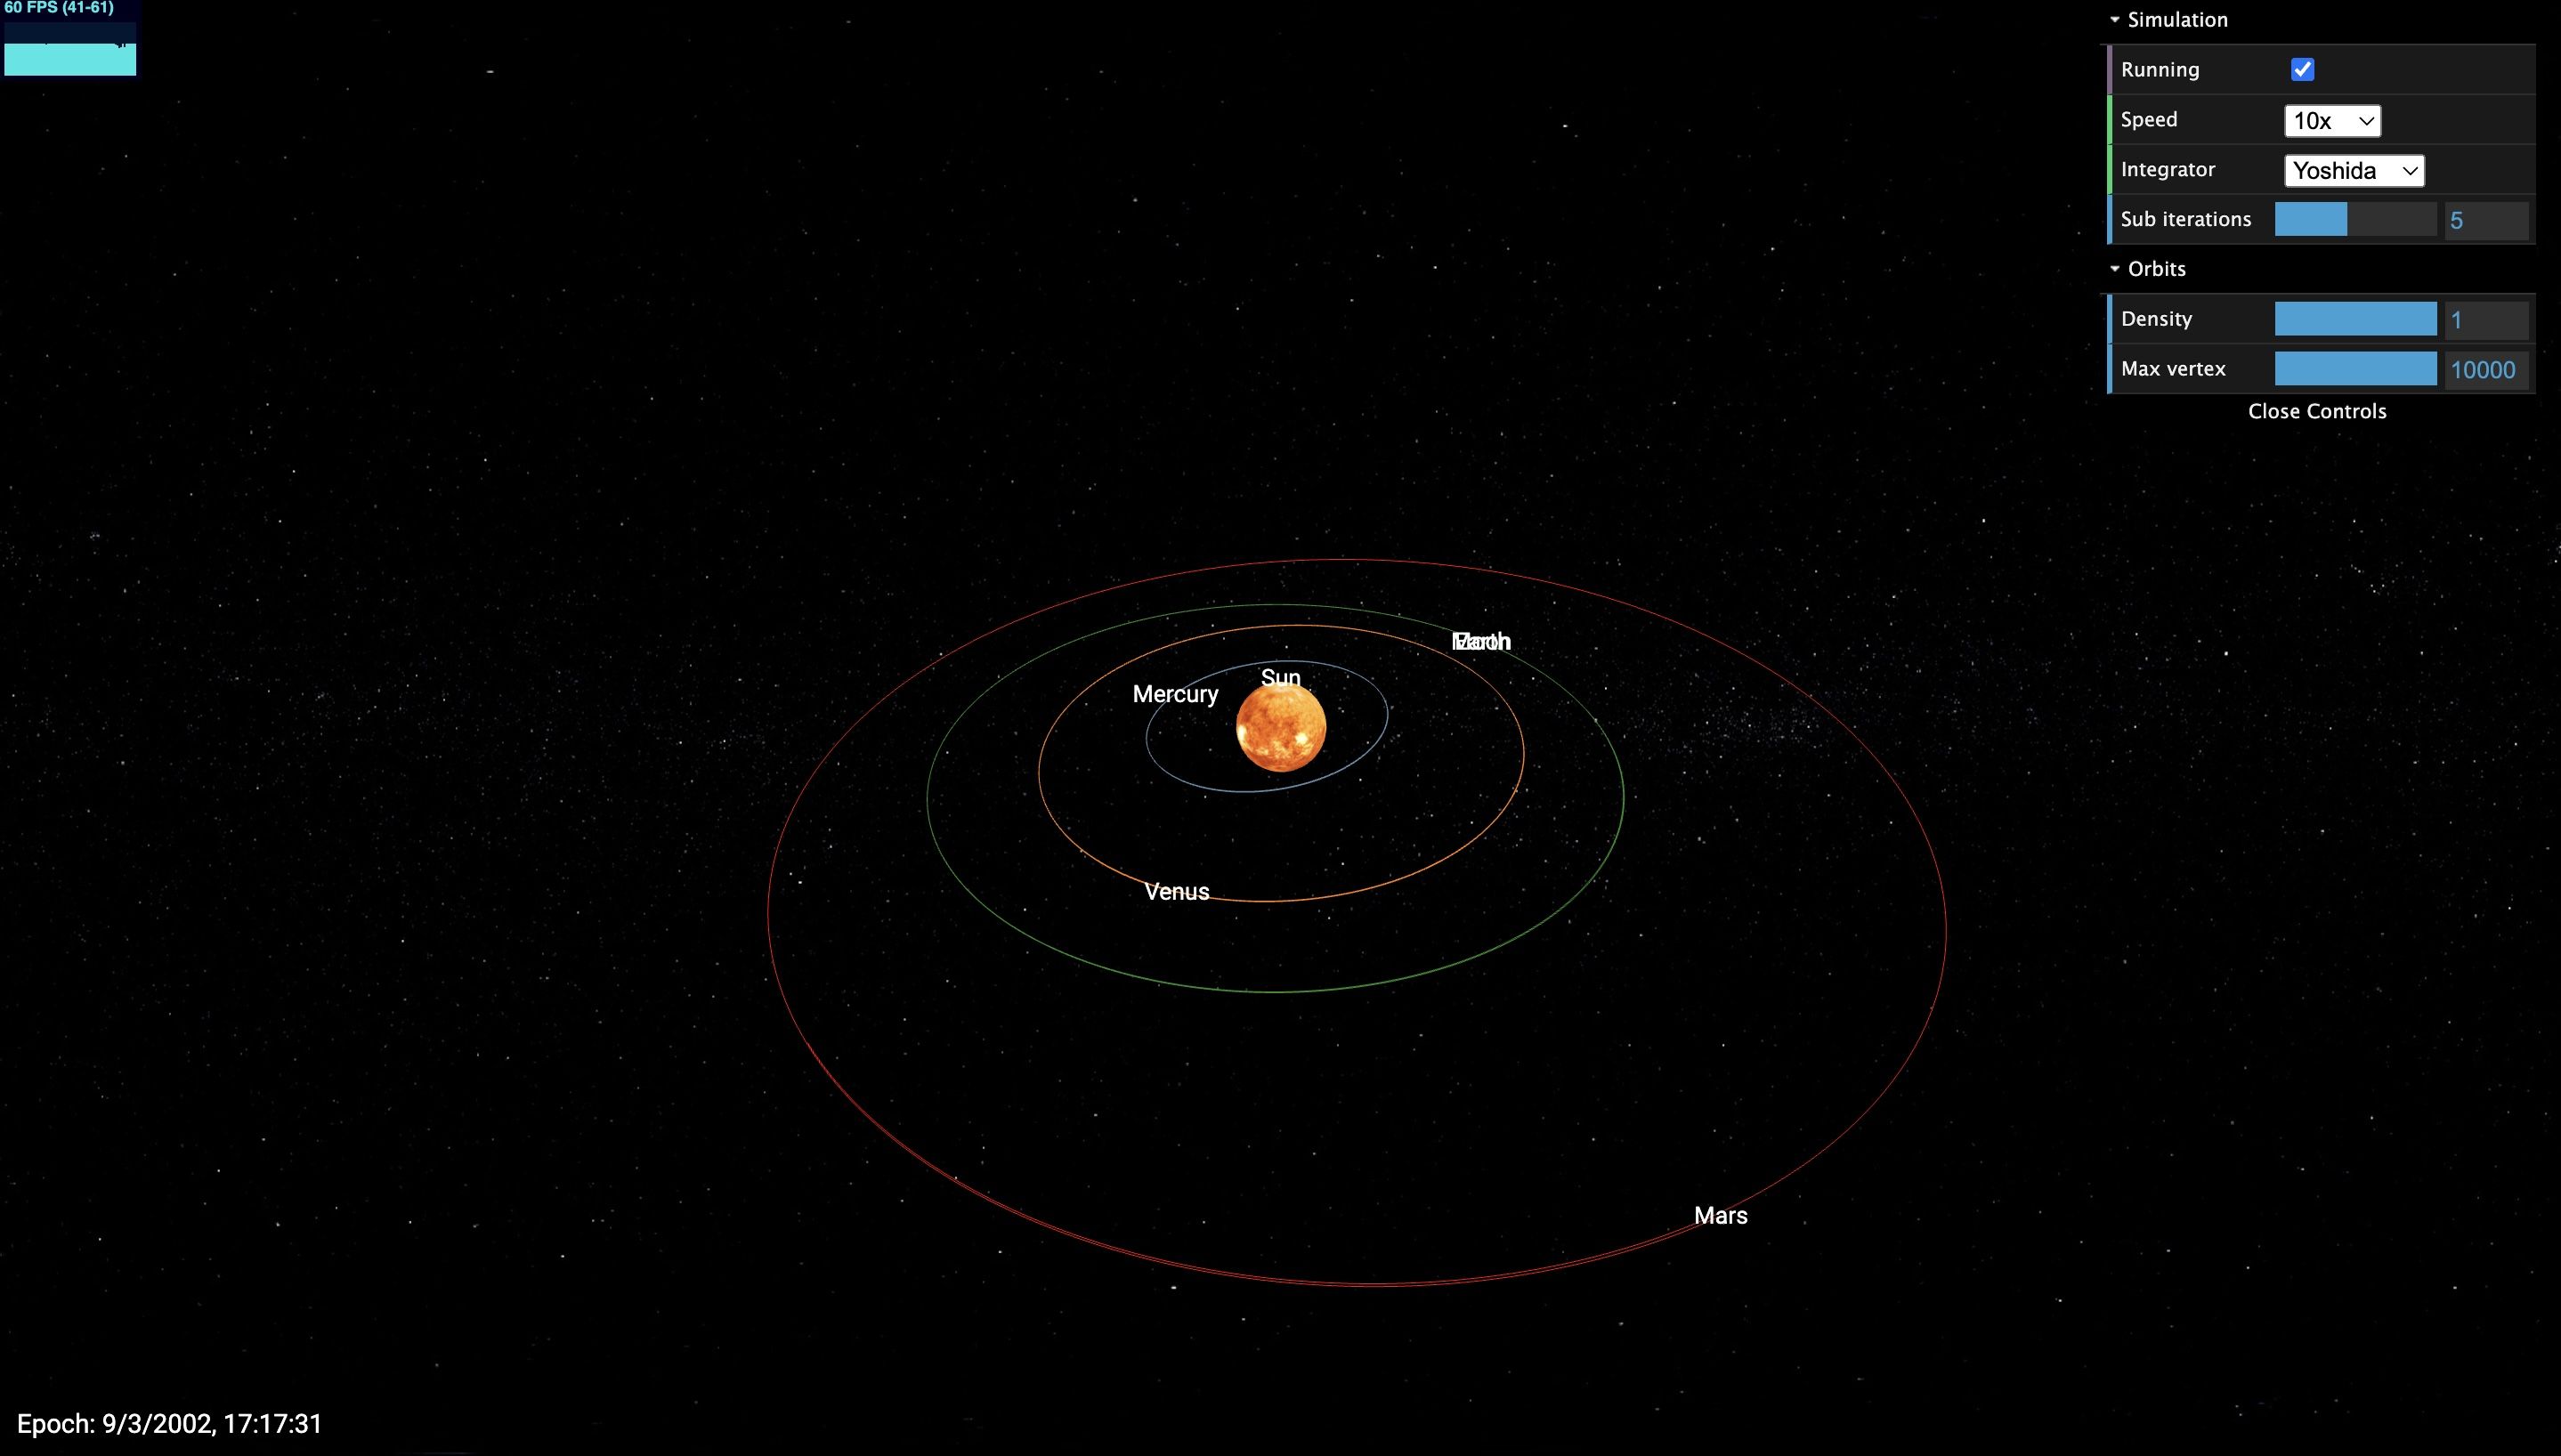
\includegraphics[width=\linewidth]{simulation_inner_planets.jpg}
		\caption{Simulazione dei pianeti interni e della Luna.}
	\end{figure}

	\section{Sviluppi futuri}

	Il codice postato in questo documento è soggetto a revisione costante e potrebbe cambiare da un momento all'altro, per risolvere bug o aggiungere funzionalità.

	Tra le modifiche più rilevanti che nel futuro verranno implementate vi è l'algoritmo di Barnes-Hut, che permette di calcolare le accelerazioni dei corpi con una complessità pari a $O(N\log{N})$, invece del corrente $O(N^2)$.

	Risulterebbe anche interessante poter lanciare dei satelliti da un pianeta direttamente dalla simulazione, selezionando latitudine e longitudine del punto di lancio e poi il beta angle.

	Infine, poiché la simulazione inizia sempre il 1 gennaio 2000, si può aggiungere la possibilità di cambiare data, sia avanti che indietro nel tempo, senza dover attendere che la simulazione la raggiunga.

	\printbibliography

\end{document}